\section{Prediction error}

To evaluate prediction quality, we define the prediction error (or residual) as:
\[\varepsilon(t+r)=v(t+r)-\hat{v}(t+r|t)\]
The optimal predictor minimizes the mean square prediction error (MSPE), which is the variance of the residual:
\[\min\left( \mathbb{E}\left[\varepsilon(t)^2 \right] \right)\]
Considering the expansion of $W(z)$ in negative powers of $z$:
\[W(z)=w_0+w_1z^{-1}+w_2z^{-2}+\dots\]
We can represent $v(t)$ as an infinite linear combination of past noise values:
\[v(t)=w_0\eta(t)+w_1\eta(t-1)+w_2\eta(t-2)+\dots\]
Assuming we have access to the past of $\eta(\cdot)$, we can estimate $v(t+r)$ for $r \geq 1$:
\[v(t+r)=\underbrace{w_0\eta(t+r)+w_1\eta(t+r-1)+\dots+w_{r-1}\eta(t+1)}_{\alpha(t)} +\underbrace{w_r\eta(t)+w_{r+1}\eta(t-1)+\dots}_{\beta(t)} \]
Here, $\alpha(t)$ and $\beta(t)$ are uncorrelated random variables, computed over non-overlapping time ranges:
\begin{itemize}
    \item $\beta(t)$ is computable once the past of $\eta(\cdot)$ (up to $t$) is known.
    \item $\alpha(t)$ depends on the future of $\eta(\cdot)$ (from $t+1$ to $t+r$).
\end{itemize}
Thus, $\alpha(t)$ shows no correlation with the past until time $t$, indicating its unpredictability based on past information.
As a result, we can estimate its mean solely, which is zero:
\[\mathbb{E}=w_0\mathbb{E}\left[\eta(t+r)\right]+w_1\mathbb{E}\left[\eta(t+r-1)\right]+\dots+w_{r-1}\mathbb{E}\left[\eta(t+1)\right]=0\]
This leads to the optimal predictor:
\[\hat{v}(t+r|t)=\beta(t)=w_r\eta(t)+w_{r+1}\eta(t-1)+\dots\]
The prediction error is then:
\[\varepsilon(t+r)=v(t+r)-\hat{v}(t+r|t)=\alpha(t)=w_0\eta(t+r-1)+\dots+w_{r-1}\eta(t+1)\]
It's noteworthy that $\varepsilon(\cdot)$ represents an MA process. 
Its mean value is 0, and its variance is $(w_0^2 + w_1^2 + \dots + w_{r-1}^2)\lambda^2$.

Furthermore, the variance increases monotonically with $r$, indicating that prediction uncertainty grows as the prediction horizon extends:
\begin{itemize}
    \item For $r=1$, the variance is $w_0^2\lambda^2$.
        When $w_0=1$ (if $W(z)$ is canonical), it matches the noise variance:
        \[\text{Var}\left[\varepsilon(t) \right]=\text{Var}\left[\eta(t) \right]\]
    \item As $r$ approaches infinity, the variance becomes $(w_0^2 + w_1^2 + \dots)\lambda^2$, equivalent to the variance of the entire process $v(t)$:
        \[\text{Var}\left[\varepsilon(t) \right]=\text{Var}\left[v(t) \right]\]
\end{itemize}
Predicting becomes increasingly challenging with larger $r$ as the estimation concerns a distant time point beyond available data. 
Over time, past data lose utility, and the most reasonable estimate is the variable's mean:
\[\mathbb{E}\left[v(t+r)\right]=0\]
Consequently, the variance of the prediction error approaches that of the process:
\[\text{Var}\left[\varepsilon(t)\right]=\mathbb{E}\left[\left(v(t+r)-\hat{v}(t+r|t)\right)^2\right]=\text{Var}\left[v(t)\right]\]
The optimal predictor can be expressed using operator notation:
\[\hat{v}(t+r|t)=\left[w_r+w_{r+1}z^{-1}+w_{r+2}z^{-2}+\dots \right]\eta(t)=\hat{W}_r(z)\eta(t)\]
To find $\hat{W}_R(z)$, observe that the transfer function can be expressed as:
\begin{align*}
    W(z)    &= w_0+w_1z^{-1} + \dots + w_{r-1}z^{-(r-1)}+w_rz^{-r}+w_{r+1}z^{-r-1}+\dots \\
            &= \underbrace{\left(w_0+w_1z^{-1} + \dots + w_{r-1}z^{-(r-1)}\right)}_{E(z)}  +z^{-r}\underbrace{\left( w_r+w_{r+1}z^{-1}+\dots\right)}_{\hat{W}_r(z)} \\
            &= E(z)  +z^{-r}\hat{W}_r(z)              
\end{align*}
Where $E(z)$ is a polynomial of degree $r-1$, and $\hat{W}_r(z)$ is a power series in $z^{-r}$ (representing a transfer function).
Thus, $\hat{W}_r(z)$ can be determined by performing long division of the numerator of $W(z)$ by its denominator, iterated for $r$ steps:
\[\hat{W}_r(z)=\dfrac{F_r(z)}{A(z)}\]
Here, $F_r(z)$ is the remainder of the division.

\subsection{Optimal predictor}
The optimal predictor we derived relies on past values of the white noise process, which may not be readily available in practice. 
Typically, we only have access to a sequence of data from the $v(\cdot)$ process. 
Let's make the following assumptions:
\begin{itemize}
    \item $W(z)$ and $\eta(t)$ represent a canonical representation of $v(t)$.
    \item $W(z)$ has no zeros on the unit circle boundary ($\Sigma(\omega)>0 \quad \forall\omega$).
\end{itemize}
Under these assumptions, we can reconstruct $W(t)$ using a whitening filter with transfer function $W(z)^{-1}$:
\[\eta(t)=\dfrac{A(z)}{C(z)}v(t)\]
The whitening filter offers a well-defined representation of $\eta(t)$ since polynomials $A(z)$ and $C(z)$ have the same degree. 
Hence, $\check{W}(z) = W(z)^{-1}$ can be interpreted as a legitimate transfer function. Moreover, $C(z)$ being a Schur-stable polynomial ensures the stationarity of the process.
\begin{figure}[H]
    \centering
    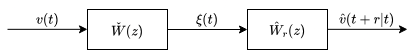
\includegraphics[width=0.75\linewidth]{images/wn.png}
\end{figure}
By combining the whitening filter with the optimal predictor derived from the noise, we obtain the optimal predictor from the process data:
\[W_r(z)=\check{W}(z)\hat{W}_r(z)=\dfrac{A(z)}{C(z)}\dfrac{F_r(z)}{A(z)}=\dfrac{F_r(z)}{C(z)}\]
The optimal predictor from $v(t)$ aligns with that from the noise, with the denominator replaced by the numerator of $\hat{W}(z)$. 
It's important to note that this predictor is also a stochastic process dependent on $v(\cdot)$, and it remains stationary.

\subsection{Predictor initialization}
Unless $C(z)$ is trivially $1$, the optimal predictor from data takes the form of a recursive equation:
\[\hat{v}(t+r|t)=-c_1\hat{v}(t+r-1|t-1)-c_2\hat{v}(t+r-2|t-2)+\dots\]
The challenge arises from having data only up to a certain instant. 
A heuristic solution is proposed: when data are unavailable, we initialize $\hat{v}$ to $\mathbb{E}[v]$ (trivial predictor).
The asymptotic stability of the filter $W_r(z)$ ensures that the effect of initialization diminishes over time.
\begin{example}
    Let's examine an MA(1) process:
    \[v(t)=\eta(t)+c\eta(t-1) \quad\eta(\cdot)\sim WN(0,\lambda^2)\] 
    where $\left\lvert c \right\rvert<1$. 
    This form implies the model is in canonical form:
    \[W(z)=1+cz^{-1}\]
    Given that the transfer function is already expressed as an expansion of negative powers of $z$, we can skip the long division procedure:
    \[\begin{cases}
        \hat{W}_1(z)=c \rightarrow \hat{v}(t+1|t)=-c\hat{v}(t|t-1)+cv(t) \\
        \hat{W}_r(z)=0 \rightarrow \hat{v}(t+r|t)=0
    \end{cases}\]
    As the covariance is null for $|\tau| > 1$, past data up to $t$ do not aid in predicting $v(\cdot)$ two or more steps ahead. 
    The only viable estimate is the mean value, which is 0. 
    Consequently, $\text{Var}[\varepsilon(t)] = \text{Var}[v(t)]$.
\end{example}
Attempting to predict a process with a model that is not in canonical form results in a non-stationary process because the model is unstable. 
Essentially, we would be trying to predict a stationary process using a non-stationary model, which is not feasible.